\documentclass[a4paper]{article}

%%%%%%%%%%%%%%%%%%%%%%%%%%%%%%%%%%%%%%%%%%%%%%%%%%%%%%%%%%%%%%%%%%%%%%
% Imports.
%%%%%%%%%%%%%%%%%%%%%%%%%%%%%%%%%%%%%%%%%%%%%%%%%%%%%%%%%%%%%%%%%%%%%%

\usepackage{amsmath,amssymb,amsfonts}  % Typical maths resource packages
\usepackage{graphics}                  % Packages to allow inclusion of graphics
\DeclareGraphicsExtensions{.pdf,.png}
\usepackage{epstopdf}				   % Package to avoid errors on .eps to pdf conversions

\usepackage{fancyhdr}				   % Redesign the header and footer
\pagestyle{fancy}
\fancyfoot{}
\fancyhead{}
\fancyhead[OR]{\thepage}
\fancyhead[EL]{\thepage}


%\usepackage[T1]{fontenc}			   % Vectoriel fonts
\usepackage[french]{babel}			   % For french quotes
\usepackage{xcolor, url}			   % For links' colour

\usepackage{color}                     % For creating coloured text and background
\usepackage{hyperref}                  
\usepackage{textcomp}

\usepackage{xcolor}

% Listings settings.
\usepackage{courier}
\usepackage{caption}
\DeclareCaptionFont{white}{\color{white}}
\DeclareCaptionFormat{listing}{\colorbox[cmyk]{0.95, 0.95, 0.95,0.01}{\parbox{\textwidth}{\hspace{15pt}#1#2#3}}}
\captionsetup[lstlisting]{format=listing,labelfont=white,textfont=white, singlelinecheck=false, margin=0pt}

\usepackage{float}
\usepackage[hyperref,framed]{ntheorem} % For creating nice definition boxes
\usepackage[all]{hypcap}
\usepackage{framed}
\usepackage{pstricks}
\usepackage{listings}                  % For code listings
\usepackage{makeidx}                   % For generating index
\usepackage{enumitem}				   % http://ctan.org/pkg/enumitem
\usepackage[nohyperlinks]{acronym}
\usepackage{Msc}

\RequirePackage[left=2.4cm,right=2.4cm,bottom=2cm]{geometry} % Redefine the page margins
%\usepackage[hmargin=2.4cm]{geometry}

\renewcommand{\labelitemi}{$\bullet$}

\renewcommand\lstlistingname{Listing}
\renewcommand\lstlistlistingname{List of listings}

%%%%%%%%%%%%%%%%%%%%%%%%%%%%%%%%%%%%%%%%%%%%%%%%%%%%%%%%%%%%%%%%%%%%%%
%\parindent 1cm
%\parskip 0.2cm
%\topmargin 0cm
%\bottommargin 0cm
%\rightmargin 0cm
%\leftmargin 0cm
%\oddsidemargin 1cm
%\evensidemargin 0.5cm
%\textwidth 15cm
%\textheight 21cm
%\makeindex

%%%%%%%%%%%%%%%%%%%%%%%%%%%%%%%%%%%%%%%%%%%%%%%%%%%%%%%%%%%%%%%%%%%%%%
%\renewcommand{\familydefault}{\sfdefault}

%%%%%%%%%%%%%%%%%%%%%%%%%%%%%%%%%%%%%%%%%%%%%%%%%%%%%%%%%%%%%%%%%%%%%%
% where are figures
\graphicspath{
  {./}
  {figures/}
  }

%%%%%%%%%%%%%%%%%%%%%%%%%%%%%%%%%%%%%%%%%%%%%%%%%%%%%%%%%%%%%%%%%%%%%%
%hyperref settings
\hypersetup{pdfauthor=Thomas Rouvinez, 
            pdftitle=HL7 Exchange Module, 
            pdfsubject=YourBookSubjectHere,
            colorlinks=true,
            linkcolor=black}

%%%%%%%%%%%%%%%%%%%%%%%%%%%%%%%%%%%%%%%%%%%%%%%%%%%%%%%%%%%%%%%%%%%%%%
% redefine some colors
\definecolor{shadethmcolor}{rgb}{0.9412,.9412,1.0000} % 
\definecolor{shaderulecolor}{rgb}{0.1529,0.2510,0.5451} % RoyalBlue 
\definecolor{lightergray}{gray}{0.95}
\definecolor{palegreen}{rgb}{0.7148,0.9219,0.6797} %pale green

%%%%%%%%%%%%%%%%%%%%%%%%%%%%%%%%%%%%%%%%%%%%%%%%%%%%%%%%%%%%%%%%%%%%%%
% define the theorem environments
% 1. definition
\theoremstyle{break}
\shadecolor{shadethmcolor}
\def\theoremframecommand{% 
\psframebox[fillstyle=solid,fillcolor=shadethmcolor,linecolor=shaderulecolor]} 
\newshadedtheorem{definition}{Definition}[section]
% 2. remark
\theoremstyle{plain} 
\theoremheaderfont{\normalfont\footnotesize\bfseries} 
\theorembodyfont{\normalfont\footnotesize} 
\theoremsymbol{\ensuremath{\clubsuit}} 
\theoremseparator{.}
\theoremindent1cm 
\theoremprework{\smallskip} 
\theorempostwork{\smallskip} 
\newtheorem*{remark}{$\rightarrow$ Remark}
% 3. seobs (software engineering observation)
\theoremstyle{plain} 
\theoremheaderfont{\normalfont\bfseries}
\theorembodyfont{\normalfont\normalsize}  
\theoremsymbol{\ensuremath{\clubsuit}} 
\theoremindent0cm 
\theoremseparator{.} 
\theoremprework{\bigskip\hrule} 
\theorempostwork{\hrule\bigskip} 
\newtheorem{seobs}{Software Engineering Observation}[section]
% 4. program output
\theoremstyle{nonumberplain} 
\theoremindent0.5cm 
\theorembodyfont{\ttfamily\small}
\theoremindent0cm 
\theoremseparator{} 
\theoremprework{\bigskip\verb}
\theorempostwork{\bigskip} 
\shadecolor{shadethmcolor}
\def\theoremframecommand{% 
\psframebox[fillstyle=solid,fillcolor=palegreen,linecolor=palegreen]} 
\newshadedtheorem{programoutput}{}

%%%%%%%%%%%%%%%%%%%%%%%%%%%%%%%%%%%%%%%%%%%%%%%%%%%%%%%%%%%%%%%%%%%%%%
% settings for the listings

\definecolor{green}{RGB}{0,180,10}
\definecolor{dkgreen}{rgb}{0,0.6,0}
\definecolor{gray}{rgb}{0.5,0.5,0.5}
\definecolor{mauve}{rgb}{0.58,0,0.82}

\lstset{
		language=Java,                % the language of the code
  		basicstyle=\footnotesize\ttfamily, % Standardschrift
        numbers=left,               % Ort der Zeilennummern
        numberstyle=\tiny,          % Stil der Zeilennummern
        stepnumber=1,               % Abstand zwischen den Zeilennummern
        numbersep=8pt,              % Abstand der Nummern zum Text
        tabsize=2,                  % Groesse von Tabs
        extendedchars=true,         %
        breaklines=true,            % Zeilen werden Umgebrochen
        commentstyle=\color{dkgreen},
        keywordstyle=\color{mauve},
    	   frame=b,         
        stringstyle=\color{blue}\ttfamily, % Farbe der String
        showspaces=false,           % Leerzeichen anzeigen ?
        showtabs=false,             % Tabs anzeigen ?
        xleftmargin=17pt,
        framexleftmargin=17pt,
        framexrightmargin=5pt,
        framexbottommargin=4pt,
        %backgroundcolor=\color{lightgray},
        showstringspaces=false      % Leerzeichen in Strings anzeigen ?     
 }

\begin{document}
\pagenumbering{roman}

%%%%%%%%%%%%%%%%%%%%%%%%%%%%%%%%%%%%%%%%%%%%%%%%%%%%%%%%%%%%%%%%%%%%%%
% Custom commands.
%%%%%%%%%%%%%%%%%%%%%%%%%%%%%%%%%%%%%%%%%%%%%%%%%%%%%%%%%%%%%%%%%%%%%%

\newenvironment{listCustom}{
 \begin{list}{{$\bullet$}}{		% type of item representation
  \setlength{\partopsep}{0pt}
  \setlength{\parskip}{0pt}
  \setlength{\parsep}{0pt}
  \setlength{\topsep}{5mm}
  \setlength{\itemsep}{1mm}		% space between items
  \setlength{\labelsep}{0.25cm} % bullet to text distance
  \setlength{\leftmargin}{2cm}  % reset margin
 }
}{
 \end{list}
}

{\setlength{\leftmargini}{2cm} 
\newenvironment{listCustomNumber}{
 \begin{enumerate}{		% type of item representation
  \setlength{\leftmargin}{2cm}  % reset margin
 }
}{
 \end{enumerate}
}

\newcommand*{\xml}[1]{\texttt{<#1>}}

\newcommand*{\webquote}[1]{\textsf{\og #1 \fg{}}}

\renewcommand{\contentsname}{Table of Content}
	
%%%%%%%%%%%%%%%%%%%%%%%%%%%%%%%%%%%%%%%%%%%%%%%%%%%%%%%%%%%%%%%%%%%%%%
% Title page.
%%%%%%%%%%%%%%%%%%%%%%%%%%%%%%%%%%%%%%%%%%%%%%%%%%%%%%%%%%%%%%%%%%%%%%

\title{User recognition on handwritten digits}
\course{Applied Signal Processing}

\author{Thomas Rouvinez\footnote{thomas.rouvinez@unifr.ch}, Didier Aeberhard\footnote{didier.aeberhard@unifr.ch}}
\professor{Dr. Andreas Humm\footnote{andreas.humm@unifr.ch}, Kai Chen\footnote{kai.chen@unifr.ch}, Hao Wei\footnote{hao.wei@unifr.ch }}
\date{May 16, 2014}


\rrno{}
\maketitle

\pagebreak


%%%%%%%%%%%%%%%%%%%%%%%%%%%%%%%%%%%%%%%%%%%%%%%%%%%%%%%%%%%%%%%%%%%%%%
% Content Table.
%%%%%%%%%%%%%%%%%%%%%%%%%%%%%%%%%%%%%%%%%%%%%%%%%%%%%%%%%%%%%%%%%%%%%%
	
\tableofcontents

\pagebreak

\pagenumbering{arabic}

%%%%%%%%%%%%%%%%%%%%%%%%%%%%%%%%%%%%%%%%%%%%%%%%%%%%%%%%%%%%%%%%%%%%%%
% Document.
%%%%%%%%%%%%%%%%%%%%%%%%%%%%%%%%%%%%%%%%%%%%%%%%%%%%%%%%%%%%%%%%%%%%%%

\section{Project description and goals}

During this project we intend to design and implement a system to match writing samples with their respective writers. To simplify the development, we only focus on hand-written digits. We create our own database of samples to identify users. The goal of this project lies in being able to quickly identify a writer based on how he/she writes digits. We implement the solution using Python(x,y)\footnote{See \url{https://code.google.com/p/pythonxy/}}, the PIL\footnote{See \url{http://www.pythonware.com/products/pil/}} library for image processing and PyBrain\footnote{See \url{http://pybrain.org/}} for as neural network library. In the following sections, we present the pipeline of the recognition process. Then each element is detailed separately from data acquisition and preprocessing, feature selection and extraction, classification and experiments. The code of the project can be downloaded from Github\footnote{Repository: \url{https://github.com/ThomasRouvinez/UserRecognizer}}.

\section{Program pipeline}

This section describes the pipeline of operations done throughout the whole process of user handwriting identification.\\

The first step consists in generating a feature vector for each digit written by a user. For each user we captured a grid of hand-written digits and each sample is cut in a separate buffer. Cutting is done in two steps: first cell by cell, then we use an automatic crop function to isolate the digits. The features are then computed on each sample and regrouped per user. The extracted feature vector of each sample is then used as input for the neural network that will be trained on the data. The results of the neural networks are tightly related to the choice of features they use as input. We could use a primary component analysis or search subsets to isolate information-worthy features, but we chose to experiment with new features.\\

We chose to use neural networks because most of the processing time required goes into training. This implies that the execution time is more suited for real-time applications. To identify the user based on an input sample, the program has to extract the features out of the sample and run them through the set of neural networks. The result will be a target output for all the users. The closest target to the user's identification key will have the most chances to be the user we are looking for.

\section{Data acquisition}

Recognition of users based on their writing requires to extract user-dependant features from the initial data. Capture of this data is performed by asking different users to write down ten times each digit from zero to nine in a grid. The grid is composed of one row per digit type and ten columns to store ten variations of each number. By doing so we ensure that the features extraction will capture more details about the user’s writing techniques and style. Also multiple initial data will ease the feature extraction as the values across the ten variations will carry more meaning rather than using a single piece of data (only one sample per digit).\\

For this project, we created a table made of regular squares to host the writing of the users. Each square is a 300 pixels wide bounding box. This was done to ensure the users do write in a defined space to ease the samples' extraction. Figure 1 illustrates the capture of ten variations of the first digits from a single user.

\vspace{1mm}
\begin{figure}[h!]
  \centering
    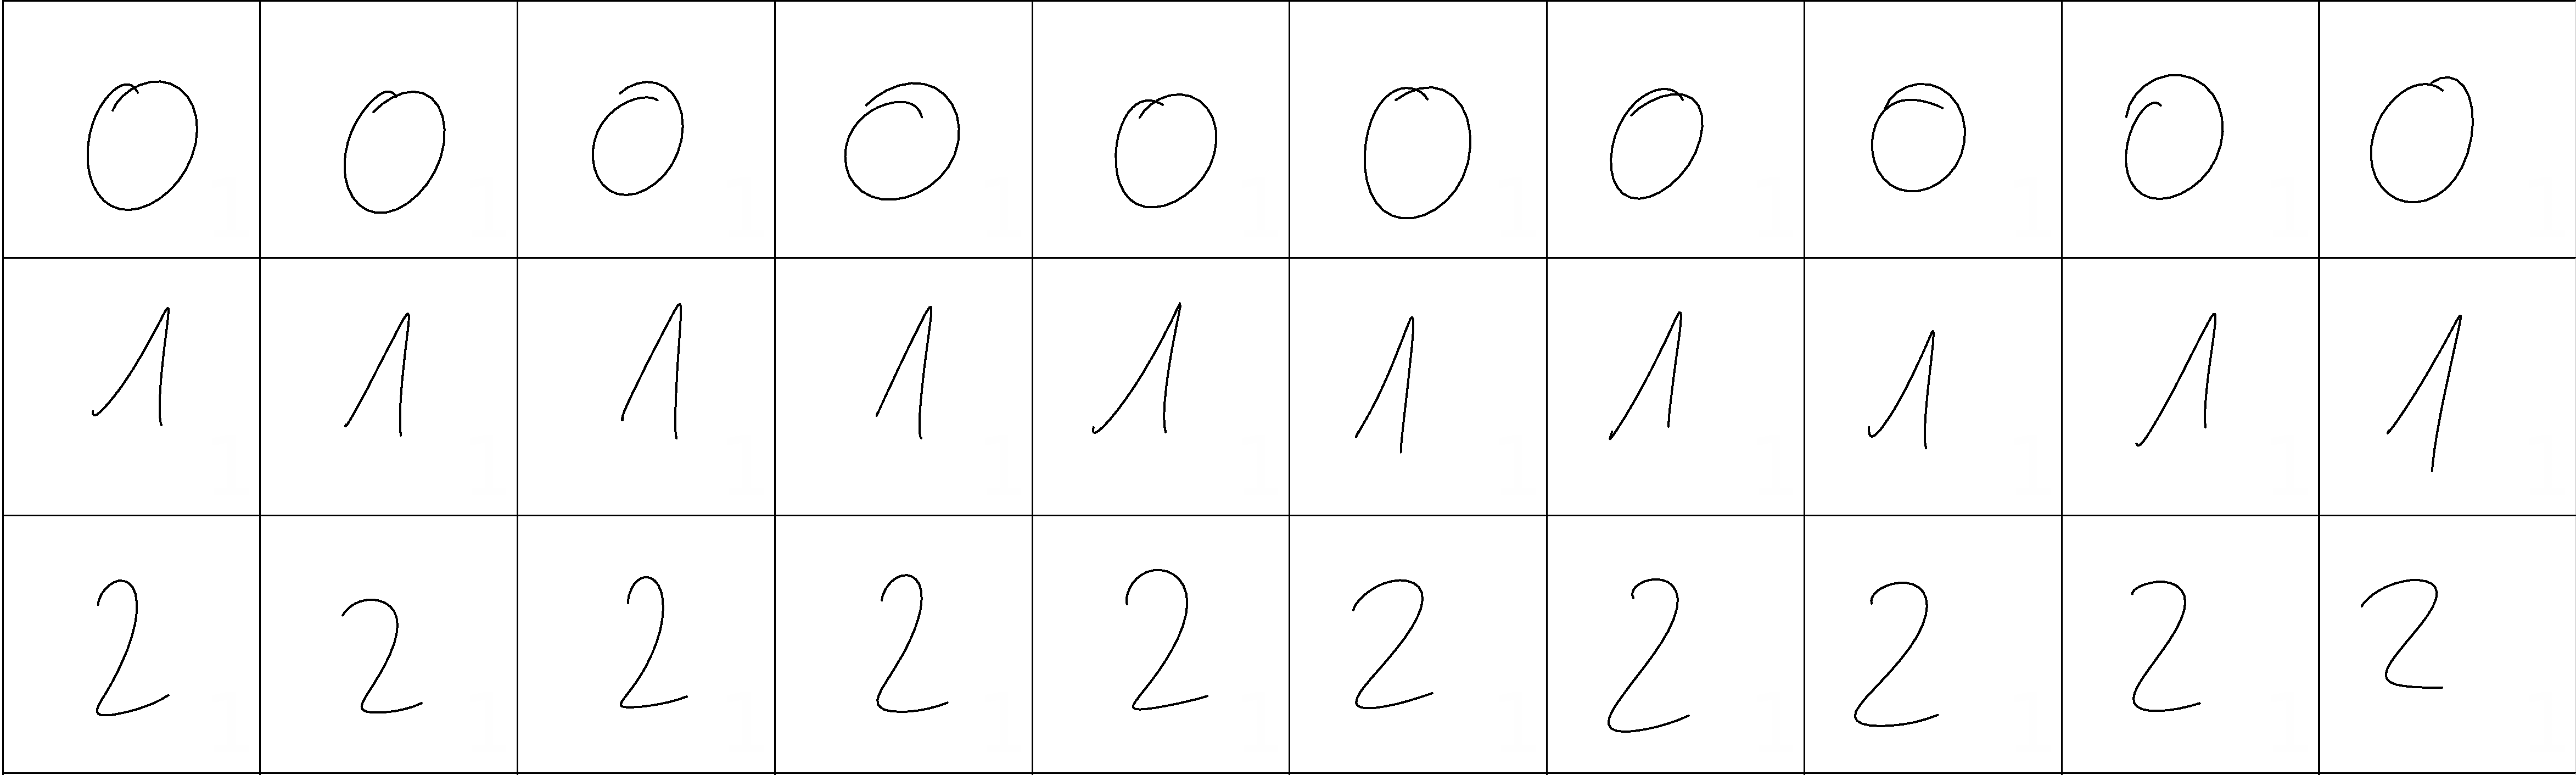
\includegraphics[scale=0.095]{didierNumbers}
  \caption{User grid example with user input.}
\end{figure}

We use offline data as it most often depicts better the real problem to solve in user recognition based on user handwriting. Such data is also harder to recognize than the online data that contains additional information. Many more features are available with online data such as writing speed and character construction patterns. Not every user starts writing letters by applying the same stroke first. Offline data does contain much information that can be turned into features, but their extraction is harder to perform: the quality of the acquired samples may vary.\\

In order to avoid capture hazards and differences that may occur by using different types of paper sheets, different pens thicknesses and colors as well as scanning jitter in quality (contrast and luminosity mostly as they can reveal or hide details), we decided to use a numerical acquisition system. We used an HP Compaq TC4200 tablet PC and asked the users to use the stylus to perform writings in the bounding boxes provided by the template grid prepared for data acquisition. This system does not influence the user’s writing as they still get to use a pen and spares extensive pre-processing on the data.\\

During the capture process, we asked all users not to write down the ten variations of a single digit at once. By allowing the users to write for example all the zeros before proceeding further on we let them become subject to involuntary repetition of features. Upon repeated writing of the same character, the human mind progressively attributes less attention to the task and this leads to a “mindless” copy of the previously done action. This contradicts our will to capture multiple variations as the results will not end up being ten variations, but maybe only two or three real variations. To counter this we required that each user fills randomly the rows or moves in diagonal only in the data grid. This resulted is a better data acquisition from a qualitative point of view as each user had to think and focus on writing another type of digit each time. We performed this process on five different users and gathered the grids of digits. On the ten variations captured per digit, we use seven for the training set of the neural networks and three for the validation set. The next section describes the pre-processing done on this data.

\section{Data pre-processing}

Data acquisition was performed digitally and thus most of the conventional pre-processing is unnecessary. In conventional cases a picture of the writing should be acquired via a scanner or camera. Then the image is converted into levels of grey to enhance contour detection and remove color variations that do not yield more useful information for features extraction. Then a combined filter of contrast and luminosity is applied to remove any glitches the digitalization process might have induced (paper quality, stains, etc). By capturing data with a tablet PC, we make sure there are only two colors (black and white) and no glitches nor noise.\\

Another set of pre-processing methods is skew and slant correction. Skew and slant represent the inclinations or the writing both horizontally considering the whole word or vertically considering each single character. In our case, skew and slant contain additional information that can translate into exploitable features for the classifier. If skew may not bring much information, slant on the other hand can provide an information on the writing speed as people tend to write more vertically the slower they write. This provides us with an online-like feature extracted from an offline sample.
\pagebreak

\section{Features selection and extraction}
\subsection{Statistical features}

Statistical features are quickly computed and extract a set of characteristics that provide global information on the samples. They can be used in combination with other types of features to assess them. Statistical features are also cheaper processing-wise.

\subsubsection{Presence}
Presence takes all the pixels and computes the percentage of black pixels compared to the surface of the sample. Despite not being the most interesting feature, it provides an idea on how much space is used by the digit in the cell. For instance if a writer is used to use curves for the lower stroke of a 2, it will increase the presence compared to another writer who uses a straight line.

\subsubsection{Mean height and width}
For each user, we compute the mean height and width per digit. We achieve this by first extracting each cell from the grid, then use PIL’s automatic crop function to isolate only the digit. Though simple, these two features already provide an information on the average size of the handwriting. Combining this information with other scale dependent features can yield interesting points to differentiate users.

\subsubsection{Center of gravity}
The center of gravity is computed by weighting the amount of black per row for the height and per column for the width. Doing so provides us with a tuple (x, y) that represent the coordinates of the center of gravity in the letter. For convenience, it is computed at the same time as presence since both features require to know the number of black pixels in the sample. The center of gravity provides information on the repartition in space of a digit.

\subsection{Structural}

Structural features require an in-depth analysis of the written digit but yield more valuable information. We are more specifically interested in learning characteristics on the writing habits of the user such as the inclination of the digits (vertically and horizontally) or the inclination of strokes and their convergence/divergence. To achieve this, we proceed by clustering the samples dynamically using horizontal and vertical splitting.

\subsubsection{Horizontal splitting}

Horizontal splitting is a known process to extract a definite amount of points in offline signatures validation. The process is the following: 

\vspace{2mm}
\begin{enumerate}
	\item Split the sample horizontally in the middle, and extract for each half the centers of gravity h0 and h1 based on the amount of writing in those areas.
	\item From h0 and h1, split vertically each horizontal half in order to get four distinct clusters in the sample.
	\item For each cluster compute the centers of gravity h2, h3, h4 h5.
\end{enumerate}
\vspace{2mm}

Once this process is done, we have extracted six points h0, ..., h5. By tracing vectors going through different combinations of these points, we extract the main features. At the end of the splitting process, we can rebuild the strokes used to draw the digit. Indeed, by tracing lines between the six points in clockwise order we can get the main strokes required to draw the digit. The order would be v2, v3, v1, v0, v4 and v5. For this project recognizing the digits is not our focus. Hence we do not recreate the tracing, but analyse the differences of angles between the major strokes. This is done with the following features:

\vspace{2mm}
\begin{listCustom}
	\item H1: angle difference between (h0,h1) and (h2,h3). With these two lines we can extract the angle difference between the mid strokes and the upper ones. With digits like 1s,  2s, 7s or 9s this difference can vary a lot from one user to the other.
	\item H2: angle difference between (h0,h1) and (h4,h5). This is the opposite of H1 as we compare the mid strokes with the lower ones.
	\item H3: angle difference between (h2,h3) and (h4,h5). It compares the angle difference between the upper strokes and the lower ones. By leaving out the mid strokes, we compute a new feature that that depicts if the user is “opening” or “closing“ his digit. By opening we mean that h3 is higher than h2 and h5 lower than h4, making the two vectors opening the area between them as we move from left to right of the sample. A “closing” digit is the opposite.
	\item H4: angle difference between (h2,h3) and an horizontal line. Since we are performing the first cut horizontally, it can become interesting to compare the upper strokes with the horizon. It yields a more neutral feature than a direct comparison between two types of strokes (upper, mid, lower).
	\item H5: angle difference between (h4,h5) and an horizontal line. Same as H4 but with the lower strokes.
	\item H6: h0 and h1 alignment. This provides a simple information on the angle of the vector that describes the mid strokes.
	\item H7: h2 and h3 alignment. This provides a simple information on the angle of the vector that describes the upper strokes.
	\item H8: h4 and h5 alignment. This provides a simple information on the angle of the vector that describes the lower strokes.
\end{listCustom}
\vspace{2mm}

\vspace{1mm}
\begin{figure}[h!]
  
  \centering
    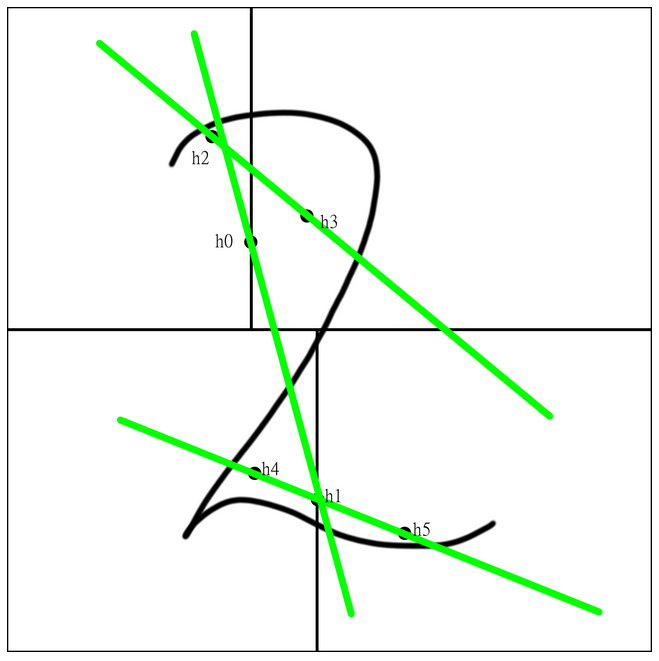
\includegraphics[scale=0.4]{hcut}
  \caption{Horizontal cuts (in black) for the digit 2, with H6, H7 and H8 dawn.}
\end{figure}

Horizontal splitting provides multiple types of information that help determining the structural differences of the writing between two users. It depicts all the six centers of gravity in the sample and are very handwriting specific. With such features we can also approximate the skew of the writing.

\subsubsection{Vertical splitting}

Vertical splitting follows the same principle as horizontal splitting but we use the notation v instead of h to differentiate both types of splits. The main difference lies in the fact that the first cut is done vertically rather than horizontally. This yields a different set of clusters of the sample and thus new features. We use the same comparisons of vectors as in the horizontal split:

\vspace{2mm}
\begin{listCustom}
	\item V1: angle difference between (v0,v1) and (v2,v3). With a vertical split first, this feature tend to provide an inverse vector compared to H1. With digits such as 8s it represents better the skew as it cuts the digit vertically in two and then V1 cuts it in an horizontal fashion, giving an approximation of the inclination of the digit. 
	\item V2: angle difference between (v0,v1) and (v4,v5).
	\item V3: angle difference between (v2,v3) and (v4,v5).  With a different original split, the centers of gravity of each cluster changes and compared to H3, V3 shows the “opening” or “closing” more on the sides of the digit (if both vectors are more or less parallel).
	\item V4: angle difference between (v2,v3) and a vertical line. This feature yields a normalization of the magnitude of the first stroke.
V5: angle difference between (v4,v5) and a vertical line. Same as V4, but for the lower strokes.
	\item V6: v0 and v1 alignment. Depicts the diagonal cut of the digit.
	\item V7: h2 and h3 alignment. 
	\item V8: v4 and v5 alignment.
\end{listCustom}
\vspace{1mm}

\begin{figure}[h!]
  \centering
    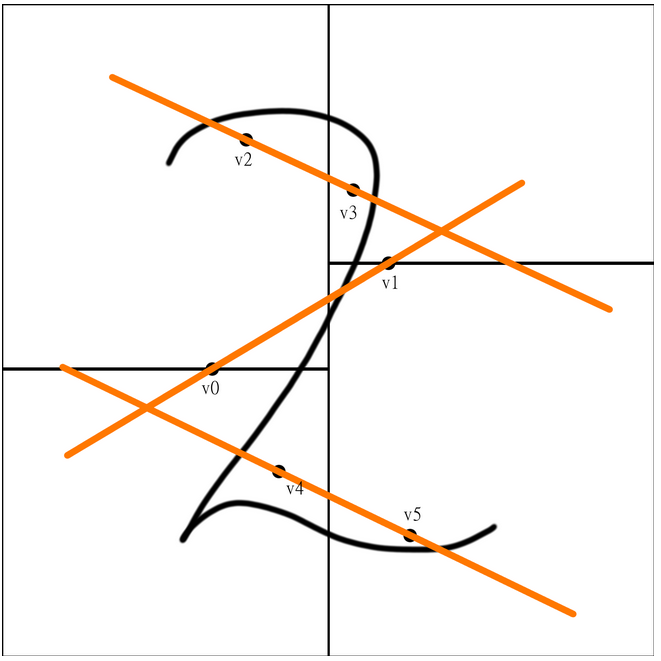
\includegraphics[scale=0.39]{vcut}
  \caption{Vertical cuts (in black) for the digit 2, with V6, V7 and V8 dawn.}
\end{figure}

Globally the horizontal features provide more information on the direction of the digit and its orientation whereas the vertical features represent more the speed, magnitude and order of the movements of the writer.

\subsubsection{Combined splitting}

Having the six centers of gravity being computed for both horizontal and vertical splits, we chose to reuse this information and gather knowledge about the differences of each type of splits. Many possibilities of comparison are possible, for example in each type of cuts we could have tried to draw lines between (v2,v4) and (v3,v5) to approximate the slant of the writing. We chose not to do so because such information may vary much between two different variations of a digit. Therefore we added the following combined features:

\begin{listCustom}
	\item C1: angle difference between (h0,h1) and (v0,v1).
	\item C2: angle difference between (h2,h3) and (v2,v3).
	\item C3: angle difference between (h4,h5) and (v4,v5).
\end{listCustom}

As seen on figures 2 and 3, the two types of cuts may generate very different distributions of the centers of gravity. Comparing them can provide precious knowledge about the writing independently from scale or variations. Note that this process could be applied further on to gain a deeper knowledge on inflection points in the writing, but for the purposes of this project and because of the size of the samples we have, we decided not to go beyond four clusters. More clusters would certainly lead to a more detailed detection of the users handwriting characteristics. In the scope of this project we tried to keep it as simple as possible to avoid long computations between two test builds. However we could imagine recursively splitting the current four clusters until the accuracy level required is reached.
\pagebreak

\section{Classifying data}
\subsection{LSTM Recurrent Neural Networks}

Once the features extraction is done for each digit variation of each user, we store them into a “Users” data object. It holds an array of “User” objects. The User object stores the name, a user-specific key\footnote{The user key is used as target output for the neural network. We then link the output of the neural network to the closest match.} and the features vectors for each digits. With this data we can now proceed with data classification in order to recognize the users.\\

We chose to use PyBrain’s neural networks library for python. It offers a wide range of neural networks including Recurrent Neural Networks (RNN) with Long-Short Term Memory (LSTM). Neural networks need to be trained on the data before they are capable of classifying it. This process takes time but allows instant execution once the training is done. We train one neural network per user. Each neural network receives seven variations from each digit of the user. Each variation is made of 24 features that are input in the neural network. We use an LSTM hidden layer of 50 neurons and a single output neuron. The networks are then trained with a back-propagation trainer and serialized for later usage. We also serialize the Users object as it represents the database of samples.\\

For this project we expect the neural networks to learn the characteristics that define the handwriting of a user. To achieve this, we have used RNNs with a memory so they can remember characteristics seen through multiple digits. Indeed the way a person writes a 1 can influence they way he/she writes a 7. There are many connections that can be established between the digits. These connections are what the neural networks should identify and work on. We have also tried multiple settings and parameters for the RNNs and found out of our experiments that increasing the momentum of the LSTM directly increased the recognition rate. This confirmed that features span across multiple digits and converge to help identify a user.\\

For more details on the settings used for the RNNs, see Chapter \ref{experimentation}.

\subsection{Post-processing}
\subsubsection{Adaptation of the activation targets}
With the first tests we have noticed that the more users there are in the process, the more deviation there was on the results. To compensate, we hard-coded a deviation function on the targets the RNNs should match. This function adds to the original target 6.25\% of it. So if a target is 3.0, when we look through the results of the RNNs we will select the closest match to 3.25. Using this temporary solution allowed us to increase the global  recognition rate from almost 10\%.

\subsubsection{User identification}
Once the results of each RNN is stored in the results array we can attempt to identify the closest match in the database. To do so we test each result of the RNNs and check which one is the closest to the requested target. To find the closest match for each result we compute the difference of the target minus the result. As this may lead to negative values, we then compute the absolute value of it and we get the "distance" to the target. We then select the smallest distance. Once this is done, we research the value selected in the array of results and take its index in the array. The index incremented by one is finally matched with all the users in the database.

\pagebreak

\section{Software manual}

In order to run this software, the following requirements should be met: first we use many libraries featured in the python(x,y) distribution such as Scypy and Numpy. PIL is integrated in Python(x,y) and does not need extra installation. However the PyBrain\footnote{Download and installation documentation: \url{http://pybrain.org/pages/download}} library should be installed separately. Once these prerequisites are installed, the software can be launched. For this purpose we use windows Powershell, but any shell supporting the execution of Python programs works. To launch the program, execute the following command in a shell:

\vspace{2mm}
\begin{lstlisting}
python .\extractor.py
\end{lstlisting}
\vspace{2mm}

Upon launch, the program will propose either to retrain the neural networks or to query them. By inputting "y" the program will take all the users as described in "extractor.py", compute the features and train one neural network per user. Note that once this process is done the program will have to be restarted to perform any queries on the database. By inputting "n", the program will ask the user if he/she wants to perform automated or manual tests (see figure \ref{guide1}). 

\begin{figure}[h!]
  \centering
    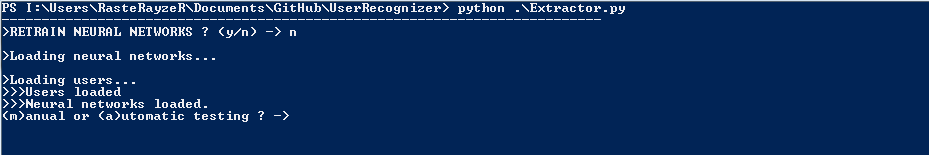
\includegraphics[scale=0.5]{guide1}
  \caption{Test mode selection (manual or automatic).}
  \label{guide1}
\end{figure}

In \textbf{manual mode}, each query requires the user to select a sample from the database. To do so, three arguments are asked: the digit to select, from which user (all users are found in ".\textbackslash Users\textbackslash username") and finally which variation of that digit should be selected. This sample is then input into the corresponding neural network and the output is returned. When possible, the output is matched with the best match known in the database. In figure \ref{guide2} we see that the user recognized is the user requested:

\begin{figure}[h!]
  \centering
    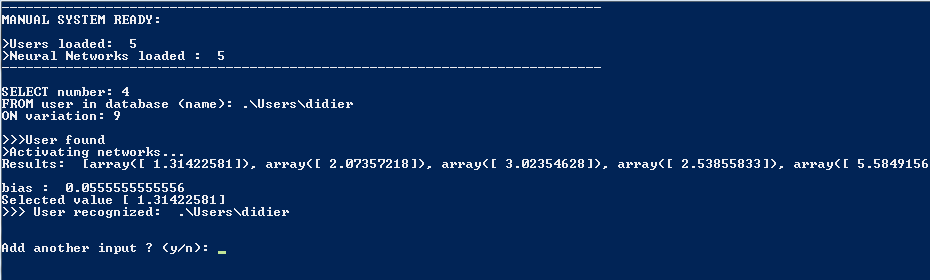
\includegraphics[scale=0.5]{guide2}
  \caption{Test mode selection (manual or automatic).}
  \label{guide2}
\end{figure}

Once a query is performed, the program offers the possibility to perform another query. By inputting 'y' you will be able to continue with this window and perform more manual queries. By inputting 'n', the program will exit.\\

In \textbf{automatic mode} the whole test set is used in the RNNs and a recognition rate is computed for each user. As visible in figure \ref{guide3}, the variations 7 to 9 of each digit are tested on all RNNs. Figure \ref{guide3} only shows the results for one user but in automatic mode all users undergo this process and return their results in the same way. For each user we indicate the name, the target the RNNs should close to as well as the recognition rate.

\begin{figure}[h!]
  \centering
    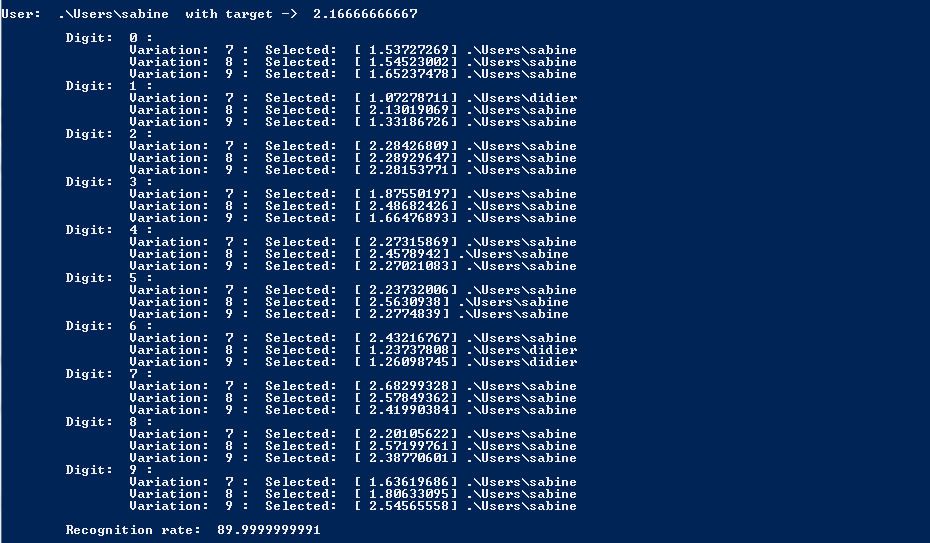
\includegraphics[scale=0.5]{guide3}
  \caption{Test mode selection (manual or automatic).}
  \label{guide3}
\end{figure}

Once the automatic mode has successfully computed and displayed all data, the program exits and leaves the results in the console. To start again tests, the user must restart the program.
\pagebreak

\section{Experimentations}
\label{experimentation}

For the experiments, we found that the following settings for the RNNs worked the best. We use a RNN with 24 inputs (one input per feature), and use a single LSTM hidden layer made of 50 neurons. Each RNN uses bias and has a single output neuron. We used 2000 epochs to train each RNN as going further leads to undesired overfitting.

\vspace{2mm}
\begin{lstlisting}
# Build the LSTM.
n = buildNetwork(24, 50, 1, hiddenclass=LSTMLayer, recurrent=True, bias=True)

# Define a training method.
trainer = BackpropTrainer(n, dataset = trndata, momentum=0.99, learningrate=0.00002)

# Carry out the training.
trainer.trainOnDataset(trndata, 2000)
\end{lstlisting}
\vspace{2mm}

Using these settings, we achieved different levels of recognition rate in the tests. This comes from the training of the RNNs not being the same at each execution. From our experimentations we have seen that a high momentum rate is drastically increasing the accuracy of the RNNs. The following results have been achieved with the best RNNs we could produce during our experiments:

\vspace{2mm}
\begin{center}
\begin{tabular}{|c|c||c|c|}
\hline 
User & Name & Target & Recognition Rate \\ 
\hline 
user01 & Didier & 1.0833333 & 99.9\% \\ 
\hline 
user02 & Sabine & 2.1666666 & 89.9\% \\ 
\hline 
user03 & Jerome & 3.25 & 93.3\% \\ 
\hline 
user04 & Pascal & 4.33333 & 99.9\% \\ 
\hline 
user05 & David & 5.4166666 & 93.3\% \\ 
\hline 
\end{tabular} 
\end{center}
\vspace{2mm}

The overall recognition rate closes to 95.26\%. Though very performant, we doubt the RNNs could achieve the same levels of recognition with more users and more variants of the digits for each user. At this point it is possible that the results obtained are overfitting the training set and happen to wonderfully fit the validation set. We retrained multiple times the RNNs and we reached an overall 82\% of recognition rate. Differences between each training were quite high but only on some users. Most of the time two RNNs would get very low recognition rates to boost only a little bit the other RNNs. We kept the globally most performant set of RNNs in the end.

\section{Improvements}

Considering the size of the project we had to make choices of implementation accordingly. The first improvement would be to use more than one classifier to perform fusion. Currently we have only the LSTM RNN with a hard-coded adaptation of the activation targets. Though the results draw 95\% of recognition rate, we have seen that the training does not always yield the same results. To counter the volatile performances of the LSTM RNN, we could use a Support Vector Machine in parallel and cross-compare the results of both classifiers. We could even imagine giving a certain weight to the classifier that performs the best.\\

Another improvement would be to actually determine a function that handles the hard-coded adaptation of the activation targets. This could be trained in another neural network or with simpler classifiers. Doing so could raise the level of accuracy of the program even more and in a dynamical way. As is we have set the best value for the current database. Though it works well up to five users, we cannot guarantee it is the case with any bigger numbers of users. Related to that we could also improve the settings of the RNN. We currently use fifty hidden neurons in one layer and it would be interesting to combine different type of hidden layers. Unfortunately such experimentations are extremely time-consuming.\\

Finally, the current console interface could be transformed in a more user-friendly GUI. Though not as important as the previous points, as we spend time in this program it shows signs of weaknesses in functionalities and ease-of-use.

\section{Conclusions}

Through this project we have acquired handwritten grids of digits for five users using a tablet PC.  We divided this data and extracted a feature vector out of each digit. Then we trained a single RNN for each user and then ran experiments on the best set of RNNs we obtained. With a recognition rate of 95\% the objective of this project is reached: recognize a user based on his/her handwriting of digits. Though extremely high, this recognition rate highly varies if the RNNs are retrained. Also we had to manually adjust  the targets of the RNNs to optimize the recognition rate. By using multiple classifiers and fusion, we hope we can achieve better results with more stability.

%%%%%%%%%%%%%%%%%%%%%%%%%%%%%%%%%%%%%%%%%%%%%%%%%%%%%%%%%%%%%%%%%%%%%%
% End of document.
%%%%%%%%%%%%%%%%%%%%%%%%%%%%%%%%%%%%%%%%%%%%%%%%%%%%%%%%%%%%%%%%%%%%%%

\end{document}